%!TEX root = ../thesis.tex
%*******************************************************************************
%*********************************** First Chapter *****************************
%*******************************************************************************

\chapter{Theory}  %Title of the First Chapter
\pagebreak

\ifpdf{}
    \graphicspath{{Chapter1/Figs/Raster/}{Chapter1/Figs/PDF/}{Chapter1/Figs/}}
\else
    \graphicspath{{Chapter1/Figs/Vector/}{Chapter1/Figs/}}
\fi


%********************************** % First Section  **************************************
\section{Rubidium} %Section - 1.1

\begin{figure}[h]
\centering
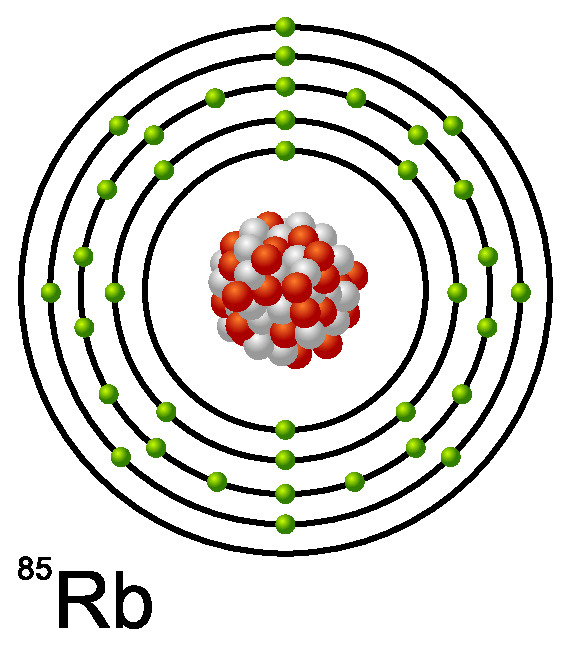
\includegraphics[width=0.3\textwidth]{rubidium_atom}
\caption[Rubidium Atom]{Schematical representation of \(^{85}\)Rb}
\label{fig:Atom}
\end{figure}

Rubidium is a chemical element with symbol Rb and atomic number 37.
It is a soft, silvery-white metallic element of the alkali metal group, 
with an atomic mass of 85.4678. Elemental rubidium is highly reactive, with 
properties similar to those of other alkali metals.\\


German chemists Robert Bunsen and Gustav Kirchhoff discovered rubidium in 
1861 by the newly developed technique, flame spectroscopy.
Because of the bright red lines in its emission spectrum, they chose a name 
derived from the Latin word rubidus, meaning ``deep red''. \citep{bunsen}\\

Although rubidium is monoisotopic, rubidium in the Earth's crust is composed of 
two isotopes: the stable \(^{85}\)Rb and the radioactive \(^{87}\)Rb. \citep{nubase}

\vspace{\fill}

\begin{table}[h]
\centering
\begin{tabular*}{0.5\textwidth}{@{\extracolsep{\fill} }l c c}
\toprule
& \multicolumn{2}{c}{Rubidium} \\
\midrule
Isotope & 85 & 87 \\
Atomic mass & 84.911794 & 86.909187 \\
in \(10^{-25}\)kg & 1.40999 & 1.44316 \\
Abundance & 72.17\% & 27.83\% \\
\bottomrule
\end{tabular*}
\caption{Properties of rubidium isotopes}
\label{table:iso_prop}
\end{table}


%********************************** % Second Section  **************************************
\section{Two-level atom} %Section - 1.2 


%********************************** % Third Section  *************************************
\section{Laser absorbtion} %Section - 1.3


%********************************** % Fourth Section  *************************************
\section{Doppler shifts}  %Section - 1.4


%********************************** % Fifth Section  *************************************
\section{Behavior of absorbtion coefficient}  %Section - 1.5


%********************************** % Sixth Section  *************************************
\section{Non-linear differential equation}  %Section - 1.6

